\documentclass{ximera}

\author{Anna Davis} \title{MTH 240 Homework 5} 

\begin{document}

\begin{abstract}

\end{abstract}
\maketitle
 \textit{Certificate due: 2/24/2021 at 11:59 p.m.}
 
 \begin{problem}\label{prob:240hom5prob5}
 Use implicit differentiation to find $\frac{dy}{dx}$ where
\[
x = y^2.
\]

\[
\frac{dy}{dx} = \answer{\frac{1}{2y}}
\]
(Author: Steven Gubkin CC-BY-NC 3.0)
 \end{problem}
 
 
 \begin{problem}\label{prob:240hom5prob4}
 Use implicit differentiation to find $\frac{dy}{dx}$ where
\[
y = \frac{x-2}{y+3}.
\]

\[
\frac{dy}{dx} = \answer{\frac{y+3}{7+x+6y+y^2}}
\]
(Author: Steven Gubkin CC-BY-NC 3.0)
 \end{problem}
 
  \begin{problem}\label{prob:240hom5prob3}
Use implicit differentiation to find $\frac{dy}{dx}$ where
\[
y^2x = \sin(xy).
\]

\[
\frac{dy}{dx} = \answer{\frac{y(y-\cos(xy))}{x(-2y+\cos(xy))}}
\]
(Author: Steven Gubkin CC-BY-NC 3.0)
 \end{problem}
 
 
 \begin{problem}\label{prob:240hom5prob6}
 Use implicit differentiation to find $\frac{dy}{dx}$ as a function of $x$ and $y$ where
\[
x^3+y^3 = 9.
\]

\[
\frac{dy}{dx} = \answer{\frac{-x^2}{y^2}}
\]

What is the equation of the tangent line to this curve at the point $(1,2)$?

\[
y = \answer{\frac{-1}{4}(x-1)+2}
\]
(Author: Steven Gubkin CC-BY-NC 3.0)
 \end{problem} 
 
 \begin{problem}\label{prob:240hom5prob1}
Find the equation of the tangent line to the curve given below at $(1,1)$.
$$xy+x^2y^2=2x$$

Start by finding $\frac{dy}{dx}$.
$$\frac{dy}{dx}=\answer{\frac{2-y-2xy^2}{x+2x^2y}}$$
Slope of the tangent line at $(1,1)$ is:
$$m=\answer{\frac{-1}{3}}$$
Equation of the tangent line is:
$$y=\answer{-\frac{1}{3}x+\frac{4}{3}}$$
 \end{problem}
 
 
 
 \begin{problem}\label{prob:240hom5prob2}
An island is located 1000 feet away from a coastal highway.  A car traveling at 88 ft/sec is approaching point $A$, as shown in the diagram.  How fast is the distance between the car and the island changing when the car is 800 feet away from point $A$?
\begin{image}
   
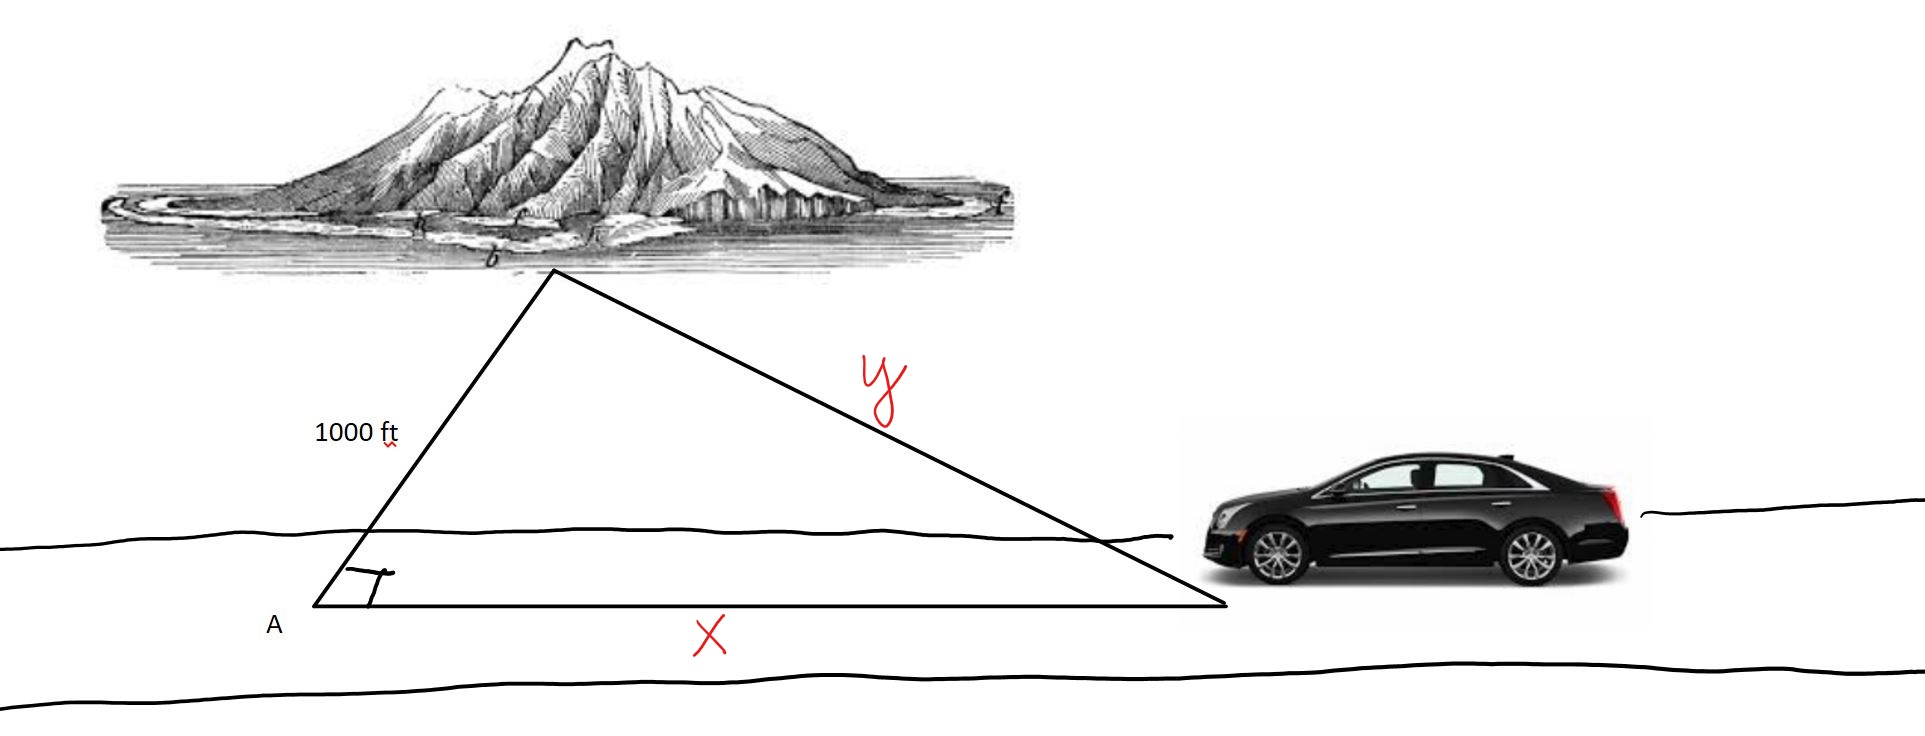
\includegraphics[height=1in]{Inkedtest2image4.jpg}~
 
\end{image}

Given rate: $\frac{dx}{dt}=\answer{-88}$.

Find rate:  $\frac{dy}{dt}$

Relationship between $\answer{x}$ and $\answer{y}$:

$$\answer{x^2}+1000^2=\answer{y^2}$$

When $x=800$, $y=\answer[tolerance=1]{1280.62}$.

The distance between the car and the island is changing at the rate of $\answer[tolerance=1]{-55}$ feet per second.
 \end{problem}
 
 \begin{problem}\label{prob:240hom5prob7}
 A $12$ foot ladder is leaning against a wall.  At the instant that the foot of the ladder is $3$ feet away from the wall, the foot of the ladder is moving away from the wall at a rate of $5 \frac{\textrm{ft}}{\textrm{s}}$.  At what rate is the top of the ladder falling down the wall at this time?

The top of the ladder is falling at a rate of $\answer[tolerance=0.1]{\frac{\sqrt{135}}{15}}$ feet per second.

(Author: Steven Gubkin CC-BY-NC 3.0)
 \end{problem}
 
 \begin{problem}\label{prob:240hom5prob8}
 A colony of bacterial are growing in a petri dish.  They form a
circular disk, which appears to be growing at a rate of $4$ square
millimeters per hour.  When the radius of the disk is $3$ millimeters,
at what rate is the radius growing?

At this instant, the radius of this disk is growing at a rate
  of $\answer{\frac{1}{2\pi}}$ millimeters each second.  (Exact answer is required; no decimal approximations.)
  
 (Author: Steven Gubkin CC-BY-NC 3.0)
 \end{problem}
 

 \end{document} 